\chapter{Regression}
Regression is a very important topic in statistics that is applied extremely
frequently. There are many different kinds of regression, but in 331 we will
mostly focus on linear regression. This gives us a nice familiar example
example to demonstrate how Bayesian statistics works and how it is different
from classical or frequentist statistics. Here we will study an example of a
simple linear regression problem taken from STATS 201.

\section{A Simple Linear Regression Problem}
Data were collected from random sample of 30 drivers. The age of the driver and the 
maximum distance at which they could read a newly designed road sign were 
recorded. It is of interest to build a simple model that can be used to predict the 
maximum distance at which the sign is legible, using the age of the driver. The file 
{\tt road.txt} contains the data. Figure~\ref{fig:road} is a plot of the data:
\begin{figure}
\begin{center}
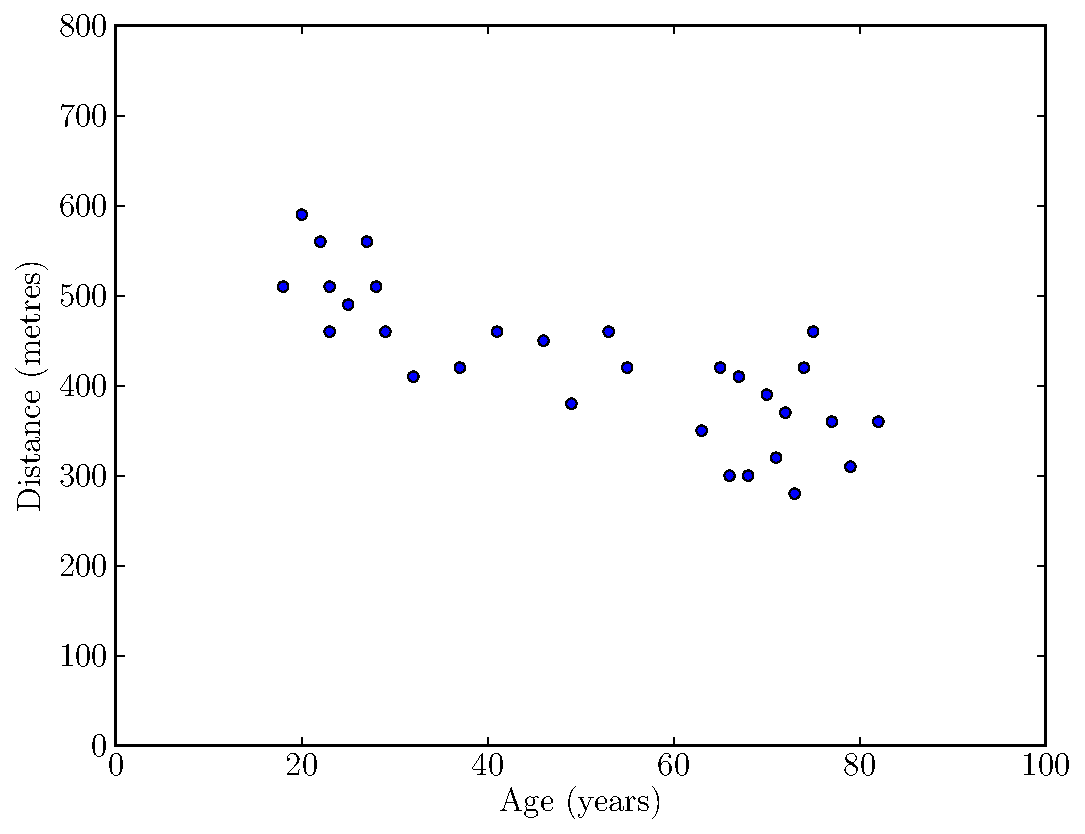
\includegraphics[scale=0.5]{Figures/road.pdf}
\caption{The distance at which a person can read a road sign, vs. the age of
the person. There are $N=30$ data points. You can clearly see that older people
have, on average, worse eyesight. But let's do a Bayesian analysis!\label{fig:road}}
\end{center}
\end{figure}
The purpose of simple linear regression is to find a straight line that goes
throught the data points. The slope and intercept of the straight line are then
helpful for understanding what is going on. Also, the straight line can be used
to predict future data, such as the maximum distance for reading the sign for a
person who is 100 years old. The most common method for obtaining the straight
line is to find the line (i.e. the slope and intercept values) that fits best
by the criterion of ``least squares''.

\section{Interpretation as a Bayesian Question}
From what you now know about Bayesian statistics, you might be able to come up
with some thoughts for what is unsatisfactory about the standard least squares
solution to linear regression. One glaring issue is that the data are {\it never
good enough} to tell us with certainty that a particular slope and intercept
are correct. In principle, we will always have uncertainty about the 


\section{Analytical Solution With Known Variance}
The unknown parameters are $\beta_0$ and $\beta_1$, and the data are the
$y$ values. Bayes' rule (parameter estimation version) will give us the
posterior distribution:
\begin{eqnarray}
p(\theta|D) \propto p(\theta)p(D|\theta)
\end{eqnarray}

Let's assume a uniform prior:
\begin{eqnarray}
p(\beta_0, \beta_1) \propto 1.
\end{eqnarray}
Now, on to the likelihood. There are $N$ data points and so there are $N$
$y$-values in the dataset. We can call those $\{y_1, y_2, ..., y_N\}$. If we
knew the true values of $\beta_0$ and $\beta_1$, then we would predict the
$y$-values to be scattered around the straight line, with the probability
distribution for the amount of scatter given by a normal distribution with
standard deviation $\sigma$, and the amount of scatter is independent for
each data point. In statisticians' notation, this can be written as:
\begin{eqnarray}
y_i \sim \mathcal{N}(\beta_0 + \beta_1 x_i, \sigma^2).
\end{eqnarray}
The full equation for the likelihood is:
\begin{eqnarray}
p(y_i|\beta_0, \beta_1) &=& \prod_{i=1}^N \frac{1}{\sigma\sqrt{2\pi}}
\exp\left[-\frac{1}{2\sigma^2}\left(y_i - (\beta_0 + \beta_1 x_i)\right)^2\right].
\end{eqnarray}
Remember that when we combine the likelihood with the prior using Bayes' rule,
we can usually ignore any constant factors out the front that do not depend on
the parameters. This allows us to ignore the first part of the product, outside
the exponential.
\begin{eqnarray}
p(\beta_0, \beta_1 | y_1, y_2, ..., y_N) &\propto& p(\beta_0, \beta_1)
p(y_1, y_2, ..., y_N|\beta_0, \beta_1)\\
&\propto& \prod_{i=1}^N \exp\left[-\frac{1}{2\sigma^2}\left(y_i - (\beta_0 + \beta_1 x_i)\right)^2\right]\\
&\propto& \exp\left[-\frac{1}{2\sigma^2}\sum_{i=1}^N\left(y_i - (\beta_0 + \beta_1 x_i)\right)^2\right].
\end{eqnarray}






\section{Solution With JAGS}
The assumption is that the data are a list of measurements:
\begin{eqnarray}
D = \{y_1, y_2, ..., y_N\}.
\end{eqnarray}
Since we are talking about linear regression, we are going to assume that the
relationship between the $x$ and the $y$ variables is described by some
straight line, but there is noise around the straight line:
The linear regression model says:
\begin{eqnarray}
y_i &=& \beta_0 + \beta_1 x_i + \epsilon_i
\end{eqnarray}
If the $\epsilon_i$ values were all zero, then the points would all lie on
a perfectly straight line.

This gives us the likelihood.

The unknown parameters are the intercept of the straight line, the gradient of
the straight line, and the standard deviation of the noise.
\begin{eqnarray}
\boldsymbol{\theta} = \{\beta_0, \beta_1, \sigma\}.
\end{eqnarray}

In JAGS, the model looks like this:
\begin{framed}
\begin{verbatim}
model
{
    # Prior for all the parameters
    beta0 ~ dnorm(0, pow(1E3, -2))
    beta1 ~ dnorm(0, pow(1E3, -2))
    log_sigma ~ dunif(-10, 10)
    sigma <- exp(log_sigma)

    # Likelihood
    for(i in 1:N)
    {
        y[i] ~ dnorm(beta0 + beta1*x[i], pow(sigma, -2))
    }
}
\end{verbatim}
\end{framed}
The first part defines the priors for the parameters. For $\beta_0$ and $\beta_1$,
we have just chosen very broad priors that describe vague prior knowledge. Note
that the standard deviations of the priors are 1000, so we should be careful
to only apply this code to situtations where we don't expect the intercept or
slope to take on an extreme value.

For the standard deviation parameter $\sigma$ which describes how much we
expect the data points to be scattered around the straight line, we have assigned
a log-uniform prior. The limits of $-10$ and $10$ for {\tt log\_sigma} imply
limits of $4.5 \times 10^{-5}$ to 22,000 for {\tt sigma}, a generous range.
Again, if we thought the scatter
was going to be outside this range, we should change the prior to something
else or risk getting strange answers.



\chapter{Simple Linear Regression With Outliers}
One complication that is common in linear regression (or other model-fitting)
problems is the existence of outliers. These are points that do not fit in with
the general trend. If these are left in the analysis, the results can easily
be incorrect. Many methods exist for deciding how to ``detect'' and ``remove''
outliers. In lectures and labs we will study and extension to the simple linear
regression model that allows for outliers. Rather than simply ``rejecting'' some
points as outliers, we can leave them in, but there will be a posterior probability
that each point is an outlier! That way, all points can contribute to the results.
Information is not wasted.



